%\documentclass[conference]{IEEEtran}
\documentclass[10pt,conference,anonymous]{IEEEtran}
\IEEEoverridecommandlockouts

%% Marcelo added this
\makeatletter
\renewcommand\footnoterule{%
  \kern-3\p@
  \hrule\@width.4\columnwidth
  \kern2.6\p@}
  \makeatother




\usepackage{inconsolata}
\usepackage{listings}

\lstset{language=Java,
basicstyle=\ttfamily\scriptsize,
%basicstyle=\ttfamily,
keywordstyle=\color{javapurple}\bfseries,
stringstyle=\color{pblue},
commentstyle=\color{javagreen},
morecomment=[s][\color{javadocblue}]{/**}{*/},
morecomment=[s][\color{gray}]{@}{\ },
numbers=left,
numberstyle=\tiny\color{black},
stepnumber=2,
numbersep=8pt,
tabsize=4,
showspaces=false,
showstringspaces=false,
breaklines=true,}

%%%%%%%%%%%%%%%%%%%%%%%%%%%%%%%%%%




\usepackage{adjustbox} % ajustar tabela ao tamanho da pagina

\usepackage{tikz}
\usetikzlibrary{matrix,fit,shapes,calc,positioning,shadows,arrows,shapes,backgrounds,decorations.markings,fadings}
\usepackage{graphicx}
\usepackage{multirow}
\usepackage[caption=false, font=footnotesize]{subfig}
\usepackage{wrapfig}
\usepackage{enumitem}
\usepackage{url}
%% helpers
\newcommand{\js}{JS}
\newcommand{\javascript}{JavaScript}
\newcommand{\es}{ES}
\newcommand{\ecmascript}{\es{}}
\newcommand{\tname}{TNAME}
\newcommand{\Comment}[1]{}
\newcommand{\numsubjects}{5}
\newcommand{\etal}{and colleagues'}
\newcommand{\ie}{i.e.}
\newcommand{\eg}{e.g.}
\newcommand{\cmark}{\ding{51}}%
\newcommand{\xmark}{{\color{red}\ding{55}}}%
\newcommand{\pGoodGood}{$\mathit{P}${\small\cmark\!\cmark}}%
\newcommand{\pGoodBad}{$\mathit{P}${\small\cmark\!\xmark}}%
\newcommand{\pBadDontCare}{$\mathit{P_?}$}%
\newcommand{\sfl}{SFL\xspace}
\newcommand{\ddg}{DDG\xspace}
\newcommand{\totfiles}{$\sim$38K}

%% annotations
\newif\ifdraftmode
%% Comment or uncomment the \draftmodetrue line.
\draftmodetrue
\ifdraftmode
 \newcommand{\Fix}[1]{\textbf{[[}{\color{red} #1}\textbf{]]}}
 \newcommand{\Mar}[1]{\textbf{[[Marcelo: }{\color{magenta} #1}\textbf{]]}}
 \newcommand{\Igor}[1]{\textbf{[[Igor: }{\color{blue} #1}\textbf{]]}}
 \newcommand{\note}[1]{\todo[inline,color=red!30,caption={}]{#1}}
\else
 \newcommand{\Fix}[1]{\relax}
 \newcommand{\Mar}[1]{\relax}
 \newcommand{\Igor}[1]{\relax}
 \newcommand{\note}[1]{\relax}
\fi

% For submitted version only.
\pagenumbering{arabic}

% Uncomment this if you need more space
%% \makeatletter
%% \def\@copyrightspace{\enlargethispage{-10pt}\relax}
%% \makeatother

\newcommand{\codesize}{\small}
\newcommand{\CodeIn}[1]{\mcodeid{#1}}
\newcommand{\CodeInM}[1]{\mcodeid{#1}}
% \|name| or \mathid{name} denotes identifiers and slots in formulas
\def\|#1|{\mathid{#1}}
\newcommand{\mathid}[1]{\ensuremath{\mathit{#1}}}
% \<name> or \codeid{name} denotes computer code identifiers
\def\<#1>{\codeid{#1}}
\newcommand{\codeid}[1]{\ifmmode{\mbox{\codesize\ttfamily{#1}}}\else{\codesize\ttfamily #1}\fi}
\def\<#1>{\mcodeid{#1}}
\newcommand{\mcodeid}[1]{\mbox{\codesize\ttfamily{#1}}}

%% thumbs up down
\newcommand*{\RightThumbsUpAux}[1]{%
  \begingroup
    \sbox0{Ag}%
    \raisebox{-\dp0}{%
      \includegraphics[{%
        height=\dimexpr\dp0+\ht0\relax,
        #1%
      }]{thumbsup.pdf}%
    }%
  \endgroup
}
\newcommand*{\RightThumbsUp}{%
  \RightThumbsUpAux{}%
}
\newcommand*{\RightThumbsDown}{%
  \RightThumbsUpAux{origin=c,angle=180}%
}
\newcommand*{\LeftThumbsUp}{%
  \scalebox{-1}[1]{\RightThumbsUp}%
}
\newcommand*{\LeftThumbsDown}{%
  \scalebox{-1}[1]{\RightThumbsDown}%
}

\newcommand{\checkm}{Y}
\newcommand{\crossmark}{N}
%\begin{wraptable}[20]{t}[0pt]{0.5\textwidth}

\newcommand{\totalTestFiles}{38,369}
\newcommand{\totalTestFilesCompileInAll}{35,939}
\newcommand{\totalTestFilesPassInAll}{24,493}
\newcommand{\nofuzzAll}{209}
\newcommand{\nofuzzBugs}{\Fix{XX}}
\newcommand{\nofuzzDuplicates}{63}
\newcommand{\nofuzzFalsePositives}{24}
\newcommand{\nofuzzHITotal}{177}
\newcommand{\nofuzzLOTotal}{32}
\newcommand{\nofuzzTotalFiles}{977} % conflicting files
\newcommand{\nofuzzFilesHI}{940} % conflicting files HI
\newcommand{\nofuzzFilesLO}{37} % conflicting files LO

\newcommand{\nofuzzBucketsBugsHI}{\Fix{124}} % buckets reported (including dups)
\newcommand{\nofuzzBucketsBugsLO}{\Fix{11}} % buckets reported
\newcommand{\nofuzzDupsHI}{\Fix{X}}
\newcommand{\nofuzzDupsLO}{\Fix{Y}}

% continue updating bugs table
\newcommand{\tableBugsNum}{\Fix{26}}

%% anonymize

\newcommand{\anonym}[1]{{\tiny\colorbox{black}{#1}}}

%% names
\newcommand{\radamsa}{radamsa}
\newcommand{\quickfuzz}{quickfuzz}

\newcommand{\jsc}{JavaScriptCore}
\newcommand{\veight}{V8}
\newcommand{\chakra}{Chakra}
\newcommand{\smonkey}{SpiderMonkey}
\newcommand{\jerry}{JerryScript}

\newcommand{\lo}{lo}
\newcommand{\hi}{hi}


\begin{document}

%Should I Fuzz my Inputs or Improve my Tests? 
\title{Differential Testing Runtime Engines--Lessons Learned from the
  JavaScript Domain}

%% \author{
%% \IEEEauthorblockN{Sabrina Souto}
%% \IEEEauthorblockA{State University of Para\'iba\\
%% Para\'iba, Brazil\\
%% sabrinadfs@gmail.com}
%% \and
%% \IEEEauthorblockN{Marcelo d'Amorim}
%% \IEEEauthorblockA{Federal University of Pernambuco\\
%%   Pernambuco, Brazil\\
%%   damorim@cin.ufpe.br}
%% \and
%% \IEEEauthorblockN{Rohit Gheyi}
%% \IEEEauthorblockA{Federal University of Campina Grande\\
%%   Para\'iba, Brazil\\
%%   rohit@dsc.ufcg.edu.br}
%% }

\maketitle

%% page numbering -M
\thispagestyle{plain}
\pagestyle{plain}

%% JavaScript (\js{}) is a popular programming language for the
%% web. Finding errors in JS runtime engines is an important problem.
\begin{abstract}
This paper assesses the impact of Differential Testing (DT) to find
functional bugs in JS engines. This is an important problem given the
importance of JS today. DT has shown successful in finding bugs in
compilers and runtimes, but has not been thoroughly explored in this
important domain. Our study \Fix{...}
\end{abstract}

\begin{IEEEkeywords}
...
\end{IEEEkeywords}

\section{Introduction}

JavaScript (\js{}) is today one of the most popular programming
languages for the web~\cite{business-insider,stackify}. The interest
of the community for the language encourages constant improvements in
its specification and implementations. It is natural to expect that
such improvements will entail sensible changes in runtime
engines~\cite{kangax}; changes that could lead to errors. Finding bugs
on JS engines is an important problem. 

Differential testing~\cite{Brumley-etal-ss07} (DT) is a popular
approach that has been applied in a variety of contexts to find
functional
bugs~\cite{Yang-etal-pldi11,Chen-etal-fse2015,Argyros-etla-ccs16,Chen-etal-pldi16,petsios-etal-sp2017,SivakornAPKJ17}. DT
automates test generation in scenarios where multiple implementations
of a system exist. It leverages the diversity across system's
implementations to detect anomalous behavior.
%% WHAT WE DID
This paper reports the results of a study we conducted to assess the
ability of DT to find bugs on \js{} engines.  We analyzed
the impact of two orthogonal dimensions: test mining and fuzzing. The
first dimension, test mining, considers the effect that \js{} test
files mined from the repository of a given open-source engine have in
detecting functional bugs in other engines. The second dimension,
fuzzing, considers the impact of fuzzing the mined files in bug
detection.
%% WHAT WE FOUND
To sum, we found that \Fix{...}

%% LIST OF CONTRIBUTIONS
This paper makes the following contributions \Fix{...}


\section{Infrastructure}
\label{sec:design}


%\begin{wrapfigure}[10]{r}[0pt]{0.45\textwidth}
\begin{figure}[t]
  \centering
%  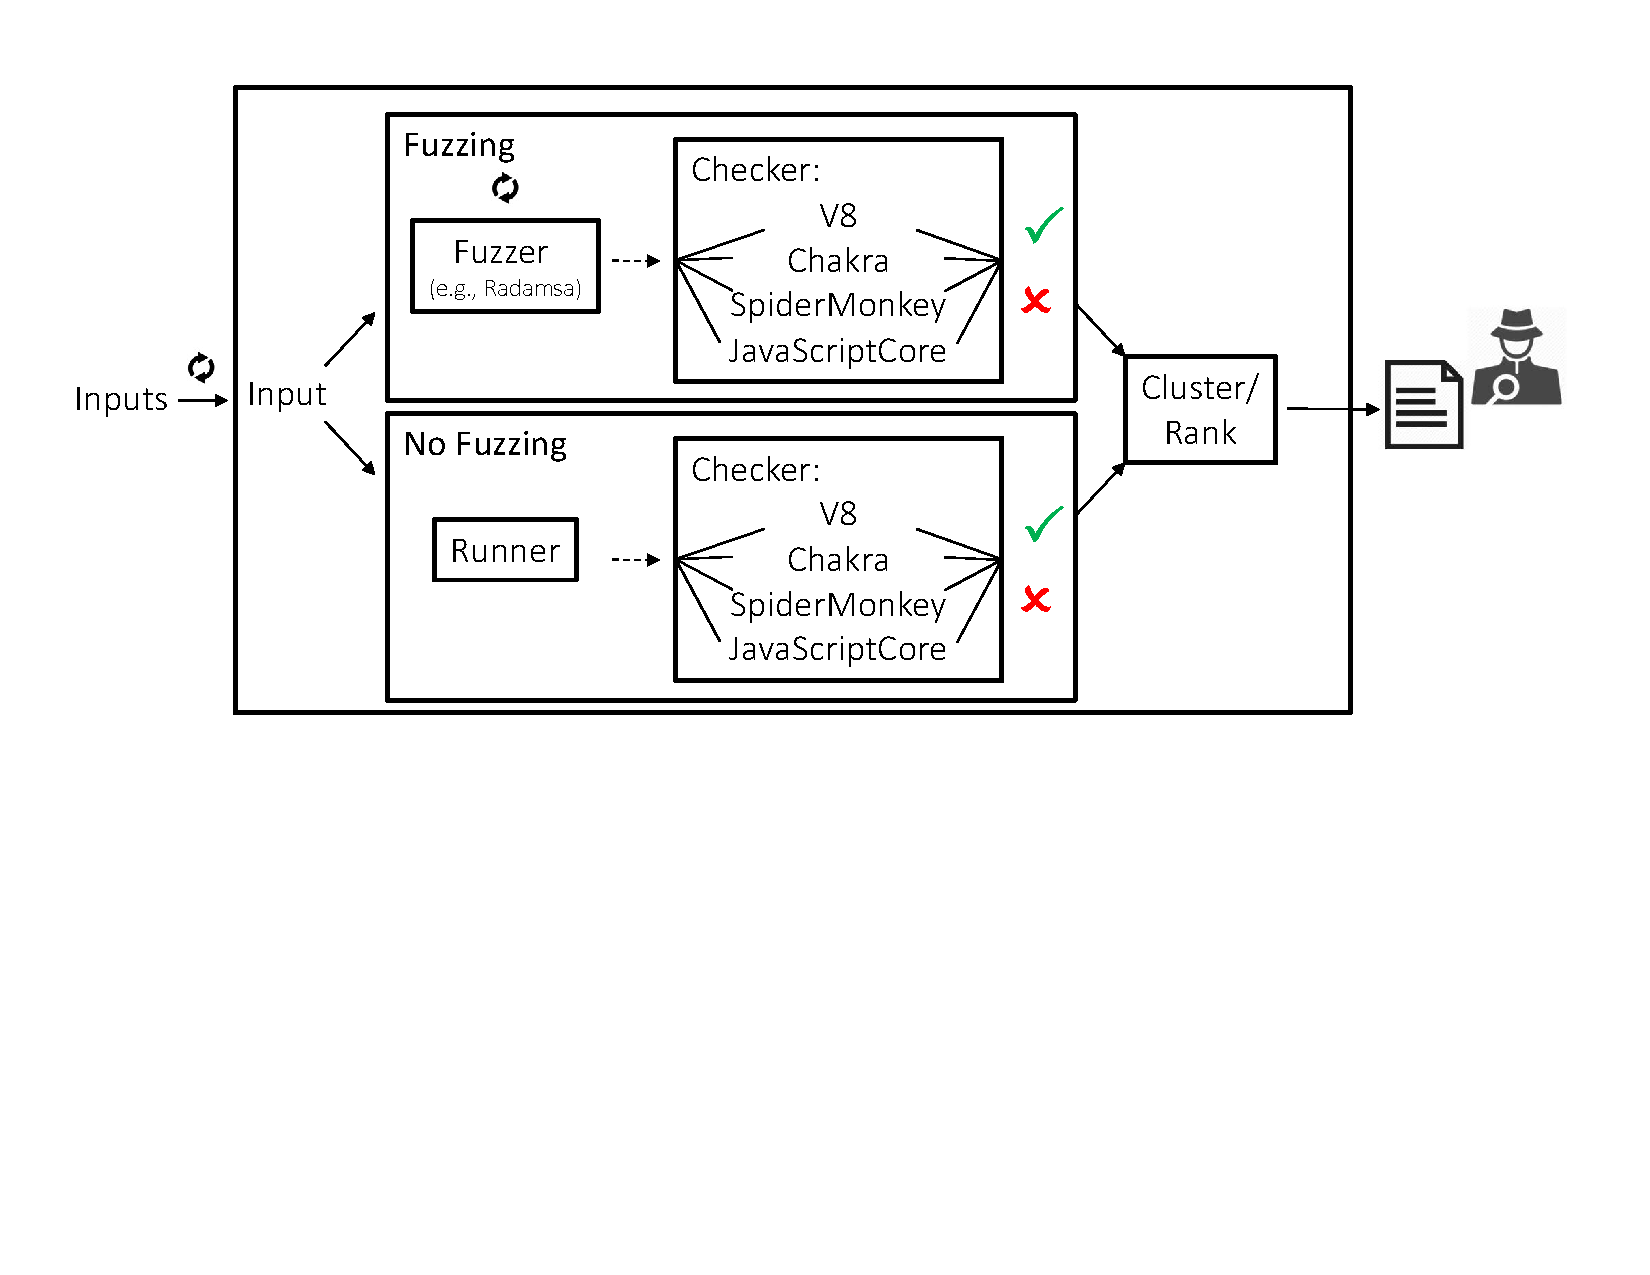
\includegraphics[trim=20 350 200
%    0,clip,width=0.35\textwidth]{google-awards-workflow}
  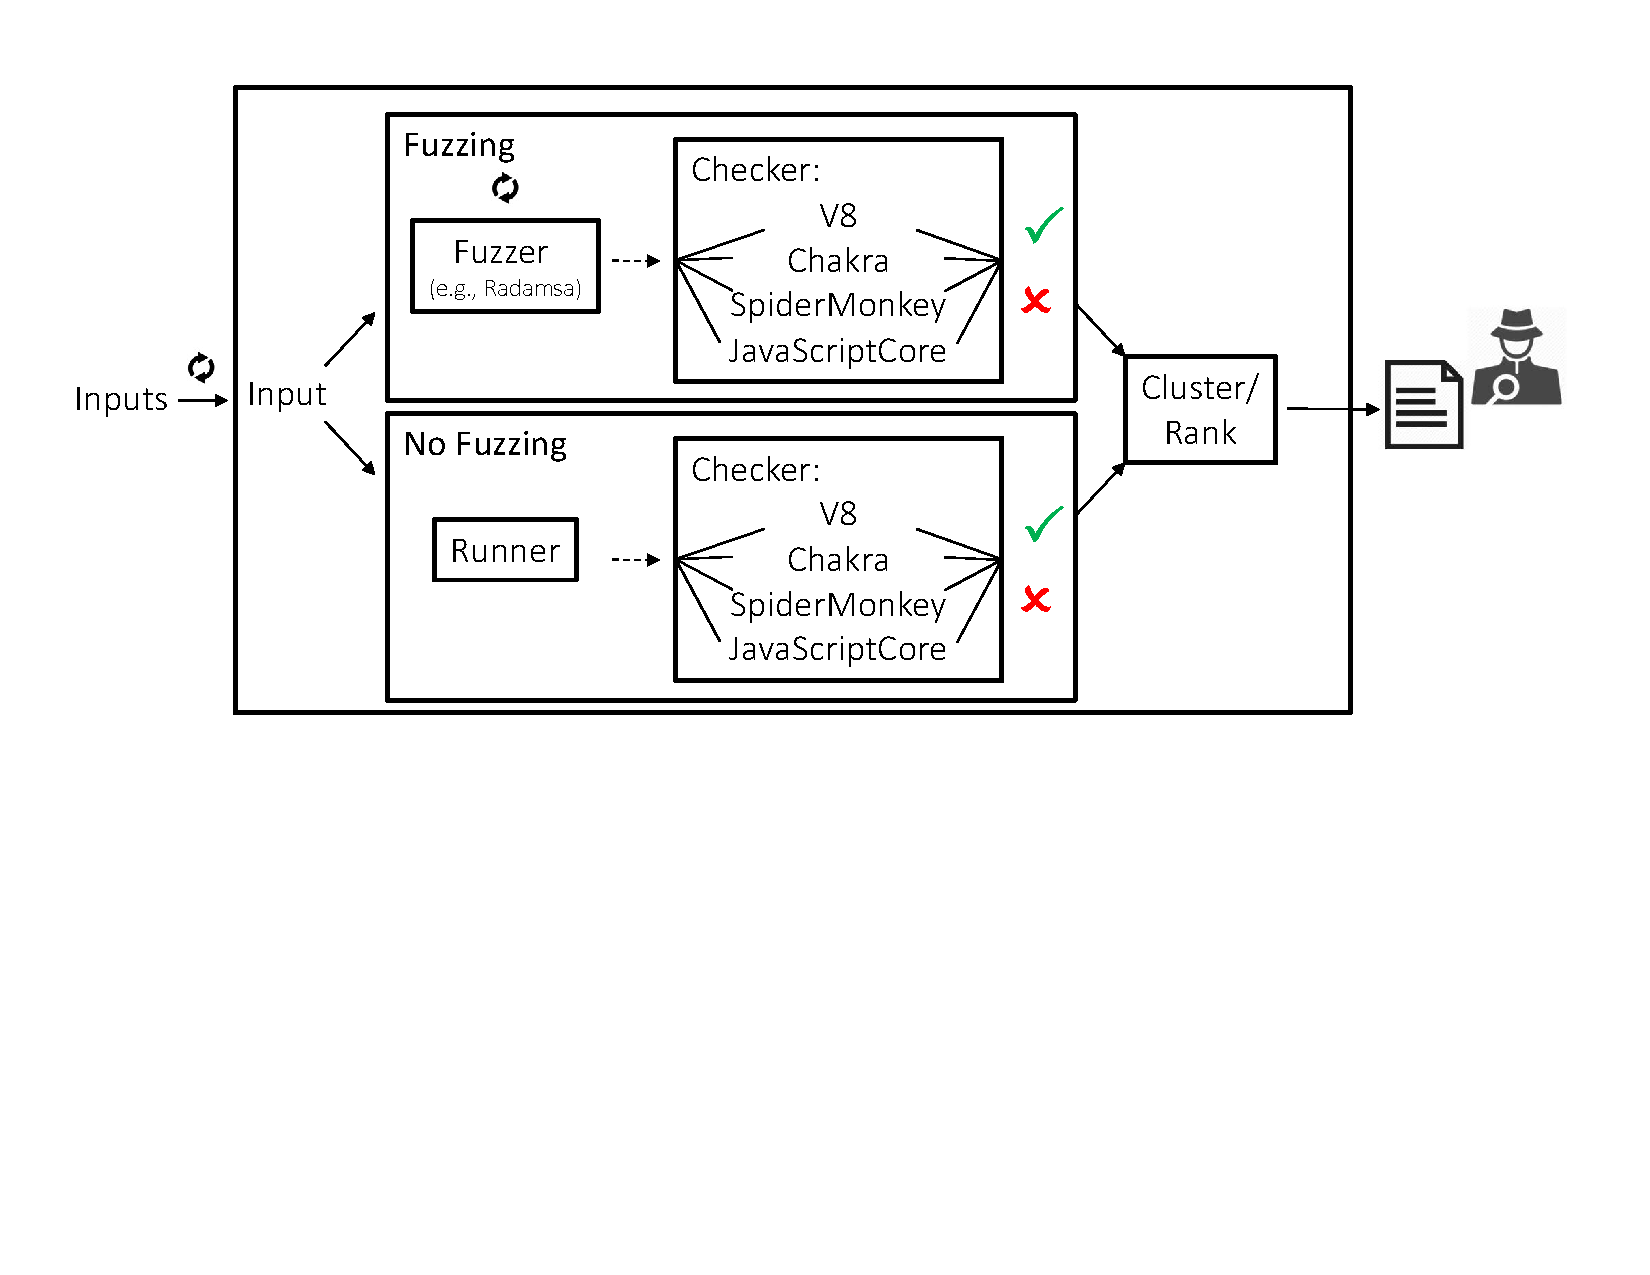
\includegraphics[trim=0 250 0 0,clip,width=0.5\textwidth]{google-awards-workflow}  
  \caption{\label{fig:workflow}Infrastructure.}
\end{figure}

Figure~\ref{fig:workflow} illustrates the infrastructure we used in
this study.
The bug-finding process
takes on input JS files from regression test suites of various JS
engines and generates warnings on output. Boxes in the figure denote encapsulation;
arrowed lines indicate control flow (dashed) and data flow
(filled). The cycle icons denote repetition--the leftmost icon
indicates that each file in the input list will be analyzed in
separate whereas the rightmost icon shows that a single file will be
fuzzed multiple times. The bug-finding process works as follows.  Considering the case
where fuzzing is not selected, as illustrated in the inner box at the bottom
of the figure, the oracle checks whether or not the output produced
for that file is consistent across all engine implementations. In case
the test passes in all engines or fails in all engines (\ie{}, the
output is consistent), the infrastructure discards the corresponding
input. Otherwise, it considers the input as potentially
fault-revealing; hence interesting for human inspection. Considering
the case where fuzzing~\cite{fuzz-testing-history} is selected, new
inputs are obtained from a given input using some off-the-shelf
fuzzer. Several fuzzing methods have been proposed in the
  past, varying with respect to how new inputs are generated (\eg{},
  coverage-based~\cite{afl,honggfuzz},
  grammar-based~\cite{grammarinator,jsfunfuzz}, and
  random-based~\cite{radamsa}). Section~\ref{sec:objects:fuzzers} describes the
  fuzzers we selected. The workflow of the infrastructure with fuzzing
  enabled is similar to that of no fuzzing. In this case, however, multiple warnings can be produced
for a given seed input.

The infrastructure outputs a list of warnings for human inspection.
To reduce the number of false alarms, we clustered warnings in two
groups, reflecting their likelihood to manifest a real bug. Warnings
in the HI group are associated with the cases when the anomaly has been
detected during the execution of the test code or its close neighborhood\Comment{ as
  opposed to that of some internal JS function}, \Igor{crashes (ie. FatalError) and core dumps 
  are considered HI group as well}. The rationale is that
the test in this group executed without violating any internal checks
of the API. In constrast, warnings in the LO group reflect the cases where the
anomaly was observed during the execution of some standard JS
function.
\Mar{is this correct? what are those?}\Igor{Yeah, it's okay}We
found that different engines often check the pre-conditions of those
functions differently. It can happen, for example, that one engine
enforces a pre-condition that another engine does not, 
% \Mar{why is that?
% that should not happen if the spec was fully documented and engines
% properly implemented those checks. Explain and give example.}
\Igor{these cases happen because the specification describes how a function
should work, however the internal implementation is defined by the engine developers}.
In those cases,
our infrastructure would observe a discrepancy that is more likely to
be associated with a bug in the (fuzzed) test; not the code. Although
we did find real bugs from warnings in the LO group, the proportion
was much lower compared to the HI group--only 12\% of the reals bugs
we found originated from the LO category. \Mar{show real examples of
  HI and LO.}
\Igor{For example, a bug caught by our environment and reported as LO priority was reported 
on Chakra engine, the JS code can be found in Figure~\ref{fig:lo-priority}. In this case,
this is a seed from Mozilla suite (\CodeIn{mozilla/non262/statements/for-in-with-assignments.js}),
the warning was not caught by the \CodeIn{assertEq} function that compares if two arguments are equals, 
the bug appears inside the generator function\footnote{Generators \url{https://developer.mozilla.org/en-US/docs/Web/JavaScript/Reference/Statements/function*}}
at line 2. According to ES6 specification\footnote{ES6 YieldExpression \url{https://www.ecma-international.org/ecma-262/8.0/index.html\#prod-YieldExpression}},
it is allowed the use of \CodeIn{yield in} in a \CodeIn{for} loop. In our infrastructure,
only Chakra engine fails with an error output \CodeIn{SyntaxError: Syntax error}, due
the output does not shows nothing related with assertions, we considered this one as a warning from LO group.
Until now, the issue was confirmed and waiting for merge/closed.
\Fix{checar ate o prazo de submissao. Essa issue esta confirmada e com commits, falta apenas o merge.}
}
\begin{figure}[h!]
  \centering
  \scriptsize
  \lstset{escapeinside={@}{@},
    numbers=left,xleftmargin=1em,frame=single,framexleftmargin=0.5em,
    basicstyle=\ttfamily\scriptsize, boxpos=c,
    numberstyle=\tiny,
    morekeywords={assertEq, var, yield, in, function},
  }
  \begin{lstlisting}
function* g1() {
  for (var x = yield in {}) ;
}
var it = g1();
assertEq(it.next().done, false);
assertEq(it.next().done, true);
  \end{lstlisting}
  \normalsize
  \caption{Bug caught by our environment as LO priority.}
  \label{fig:lo-priority}
  \end{figure}

An example of a warning from the HI group is defined in Figure~\ref{fig:hi-priority}. 
This is a testcase from WebKit.es6 suite that it was mutate by radamsa fuzzer, the 
initial seed has in line 3 the code \CodeIn{"foo".repeat(3)} but the fuzzer changed the 
integer 3 to a big integer number. We reported this case in chakra due a core dumps that occurs
during the runtime, however this case was rejected due \CodeIn{incompatibility by design} that
this is an intentional behavior of engine that crash the process if it runs out of memory
\footnote{Chakra issue \#4979 \url{https://github.com/Microsoft/ChakraCore/issues/4979}}.

\begin{figure}[h!]
  \centering
  \scriptsize
  \lstset{escapeinside={@}{@},
    numbers=left,xleftmargin=1em,frame=single,framexleftmargin=0.5em,
    basicstyle=\ttfamily\scriptsize, boxpos=c,
    numberstyle=\tiny,
    morekeywords={assertEq, var, yield, in, function, 
    typeof, return, throw, new, Error, if},
  }
  \begin{lstlisting}
function test() {
  return typeof String.prototype.repeat === "function"
    && "foo".repeat(657604378) === "foofoofoo";
}
if (!test())
  throw new Error("Test failed");
  \end{lstlisting}
  \normalsize
  \caption{Warning captured as HI priority.}
  \label{fig:hi-priority}
  \end{figure}

\Mar{can we detect dups mining issue trackers?}
\Igor{
  acho que encontrar duplicatas seria um estudo a parte, devido a linguagem natural.
  Tenho umas consideracoes:
  \begin{itemize}
    \item warning HI possui a msg "Error: Test Failed", nao tem como buscar algo com isso, 
    se for pegar a linha que falhou, provavelmente vai mostrar a linha onde o assert se encontra.
    \item warning LO: podemos tentar conseguir buscar pelo output/funcao que falhou,
    \item O fuzzinator tem algo similar (dei uma olhada rapida, nao eh complicado)
  \end{itemize}
}

\section{Objects of Study}
\label{sec:methodology}

This section discusses the objects we used in our study.

\subsection{Engines}
\label{sec:methodology:engines}~We selected the most popular JS
engines on the web~\Fix{cite} to focus our bug-finding efforts, namely
Microsoft's Chakra~\cite{chakra2018repo}, Google's
v8~\cite{v82018repo}, Mozilla's
SpiderMonkey~\cite{spidermonkey2018repo}, and Apple's JavaScriptCore
(WebKit)~\cite{jsc2018repo}.

\subsection{Seed JS files\label{sec:seeds}}~We considered test suites
associated with all four JS engines we analyzed
(section~\ref{sec:methodology:engines}). In addition, we mined tests
from other GitHub repositories based on the following selection
criteria--the project must have received at least 1K stars and the
project must not use external libraries. Figure~\ref{fig:query}
illustrates the GitHub API query~\cite{github-rest-api} we used to
find javascript engines projects defined by the label
``javascript-engine''.  The resulting list included a total of 33 projects.
\Igor{
  Due the GitHub does not supports to get the repository files via API, we
  analyzed manually each of them. It was observed that sixteen projects
  are invalid for us due the uses NodeJS that our engine cannot support it,
  empty repositories and browser support as well and another 13 projects 
  does not have a test module in their repository.
  A total of 4 projects remained after the manual inspection, two of them
  are added before, for example the V8\footnote{The official mirror of the V8 Git repository \url{https://github.com/v8/v8}}
  and V7\footnote{V7 Embedded JavaScript engine \url{https://github.com/cesanta/v7}} repositories.
  The Duktape and JerryScript tests are the seeds that we integrate on our infraestruture.
  The repositories of JSI and TinyJS are found manually and was incorpored also even less 1K of stars.
}

\begin{figure}[h]
  \centering
  \begin{lstlisting}
https://api.github.com/search/repositories?q=javascript-engine+stars:>=1000
  \end{lstlisting}
  \caption{\label{fig:query}
  Query used to find JS engine projects with over 1K stars.
  }
\end{figure}

Table~\ref{tab:test-suites} shows the JS sources we considered for
each of the selected projects.\Mar{identify the sources assoc. with
  the four analyzed engines. you said in the first sentence this is
  one source.}  Overall, we found a total of \totfiles{} JS
files.\Mar{Briefly explain these sources.} It is worth noting that some projects use distinct frameworks for
testing and require external libraries to run their testing
suites. For these projects, we needed to make small changes in the testing
infrastructure to be able to uniformly run tests in all
engines.\Mar{not entirely clear what you did to support
  this.$\rightarrow$}\Igor{wip}\Mar{apenas explique o que fez (mesmo
  que em portugues). isto
  nao deveria levar tempo que justifique escrever wip.}We aimed to use only the JS file with minor fixes
to support our environment. These fixes are composed by an assertion
function that throws an Error that we can capture by our
infraestruture.

\begin{table}[t]
  \centering
  \caption{\label{tab:test-suites}Test Suites\Mar{try to use a single
      name (if possible) to facilitate reference in the paper. Use the
  full path in the URL (citation) to indicate where one can find those
  files.}}
  \begin{tabular}{ccr}
    \toprule
    TestSuite & Source & \# JS files \\
    \midrule
    Duktape & \cite{duktape} & 997 \\
    JerryScript & \cite{jerryscript} & 1,803 \\
    JSI & \cite{jsi} & 99 \\
    Tiny-js & \cite{tinyjs} & 44 \\
    Mozilla & \Fix{??} & 32,414 \\
    V8.test.benchmarks.data & \Fix{??} & 64 \\
    WebKit.jstests.es6 & \Fix{??} & 605 \\
    WebKit.jstests.microbenchmarks & \Fix{??} & 426 \\
    \midrule
     &  & 36,452 \\
   \bottomrule     
  \end{tabular}
\end{table}

% For example to run the JerryScript tests it was necessary 
% use the unit-test package to run it, but with our changes we added the assertion
% does not have an assertion in the test file
% \Fix{add code to explain}

\subsection{Fuzzers}
\label{sec:objects:fuzzers}

In the following, we describe the list of fuzzers we analyzed. We
initially considered generational grammar-based fuzzers and mutational
fuzzers.

Grammar-based fuzzers generate a new file using the grammar of the
language whose inputs should be fuzzed. Intuitively, those fuzzers
implement a traversal of the production rules of the input grammar to
create syntax trees, which are then pretty-printed. Consequently, this
approach produces inputs that are syntatically valid by construction.
We analyzed two grammar-based
fuzzers--Grammarinator~\cite{grammarinator} and
QuickFuzz~\cite{grieco2016quickfuzz}.  Unfortunately none was
effective out of the box. Given the bound limits we defined, we were
unable to find any discrepancy in the inputs those tools generated. To
sum, the tools produced a high percentage of semantically-invalid
inputs such as \Fix{give one or two concrete examples--variable usage
  without definition?} that we needed to discard and the valid inputs
manifested no discrepancies. For example, we produced 10K inputs with
Grammarinator and only \Fix{X} were valid. With QuickFuzz, we were
able to produce \Fix{Y, Y$>$Y?} valid inputs as it contains some
heuristics to avoid generation of semantically-invalid
inputs. Nonetheless, running those inputs in our infrastructure we
were unable to find discrepancies. Inpecting the valid inputs we found
that they produced only very simple inputs. \Mar{are there weights
  associated with production rules besides the depth you can set?}

%% Our
%% infrastructure supports any grammar fuzzer with a few
%% adjusts. However, we try to integrate several grammar-based fuzzers,
%% for example
%% and \Fix{others fuzzers} to
%% generate new JavaScript files based on grammar, but after several runs
%% it was observed that this approach was ineffective due the amount of
%% invalid files and/or files without discrepancies.
%% For example, if we
%% ran Grammarinator to generate 1K JS files ten times with a random seed
%% generation, we obtained \Fix{XX\%} of valid files. Checking in our
%% environment almost \Fix{XX\%} are js files that shows undefined
%% variables and due the differential testing in our environment all
%% engines will raise a SyntaxError and this approach was not relevant to
%% our experiment.

%% We initially considered used representatives of popular fuzzing approaches. For
%% random-based fuzzing we used Radamsa~\cite{radamsa}; for
%% coverage-based fuzzing we used
%% \Fix{AFL~\cite{afl}/libfuzzer~\cite{libfuzzer}?}, and for
%% generative-based fuzzing we used
%% \Fix{grammarinator,jsfunfuzz?}. Details on how these fuzzers work can
%% be found elsewhere~\cite{fuzz-bart}.

Mutational fuzzers can be either white-box (coverage-based) or
black-box. Coverage-based fuzzers like American Fuzz Loop
(AFL)~\cite{afl} and libfuzzer~\cite{libfuzzer} run tests inputs
against instrumented versions of the program under testing with the
typical goal of finding univeral errors like crashes and buffer
overflows. The instrumentation adds code to collect coverage and
monitor properties\footnote{ There are options in the clang toolchain
  to build programs with fuzzing
  instrumentation~\cite{libfuzzer}. clang provides several sanitizers
  for property checking~\cite{clang-documentation}.}. The typical
approach to input generation is evolutionary--these fuzzers try to
minimize the distances to still-uncovered branches of the
program. AFL, for instance, takes the instrumented program binary
(say, a JS engine) and one seed input to that program (say, a JS
program) and produces on output fault-revealing inputs. Considering
our context of application, we needed to instrument one runtime engine
for fuzzing; we chose v8 for this. Unfortunately, we found that most
of the inputs produced by AFL violate the JS grammar. Furthermore, the
fuzzing task took days even when considering only one seed and there
is no simple way to guide the exploration. That happens because the
fuzzer aims to explore the entire decision tree induced from the
engine's main function, including the branches associated with the
lexer and the parser. For that reasons, coverage-based fuzzers were
not considered in this study. It is worth mentioning that Google
mitigates that problem by promoting developers to create fuzz targets
for specific program functions\Fix{cite}. Although that approach has
shown very effective, it requires domain knowledge to create the
calling context to invoke the fuzz target.

\Fix{...do the same as above for black-box fuzzing. explain what kinds of
inputs they can generate.}


\section{Results}
\label{sec:results}

In this study, we analyzed the impact of two orthogonal dimensions in
bug finding: test mining and fuzzing. The first dimension focuses on
the impact of new inputs in bug finding whereas the second dimension
focuses on the impact of variations of existing inputs in bug finding.

\subsection{Test Mining}

In this experiment, we ran all tests (see Section~\ref{sec:seeds})
using our infrastructure in no-fuzzing mode. We inspected all warnings
reported by our tool and, for those we found suspicious, we filed a
bug report in the corresponding bug tracker.

\Igor{  
  Nosso estudo revelou que dos \Fix{19} bugs reportados pelo nosso time, 
  apenas 8 nao foram fuzzados \Fix{42.1\%}, isso se da 
  a importancia tanto de utilizar fuzzing em arquivos de teste do proprio projeto,
  quanto em projetos distintos de mesma ordem, pois neste caso engines JS 
  devem interpretar arquivos, entao quanto mais entradas, melhores os resultados.
  \Fix{discuss}
}

%% \Fix{nao entendi muito sobre essa subsection... 
%% seria explicacao do porque utilizar o fuzzing baseado nos nosso resultados?}
%% \Igor{
%%   Os engines JS mais populares foram arduamente testados ao longo dos últimos anos, 
%%   o sistema robusto nao significa que esta livre de bugs, ao contrario,
%%   estamos testando-o com simples entradas a partir de testes de regressao 
%%   de bugs previamente encontrados, porem estas entradas poderiam servir como seeds 
%%   para novos testcases. Partindo disso, realizar fuzzer em arquivos 
%%   existentes em projetos open-sources eh uma maneira de
%%   aumentar ainda mais a eficiencia destes engines, por exemplo o Google incentiva o 
%%   uso de fuzzers no seu ecossistema\cite{oss-fuzz,honggfuzz}.



\subsection{Fuzzing}

The rationale for considering fuzzing as a dimension of study is to
assess the extent to which changing existing inputs helps in finding
new bugs. We measured this ability both in absolute terms and
relatively to the number of bugs found with the seed inputs in
no-fuzzing mode.

\Igor{
  Para realizar nossos experimentos, tivemos que decidir qual as 
  melhores abordagens para aumentar a efetividade dos fuzzers.
  Os fuzzers mutacionais se mostraram mais eficientes em relacao
  aos fuzzers geracionais, entao focamos neste ponto.
  Utilizamos os fuzzers radamsa, QuickFuzz e \Fix{others} nas suas configuracoes
  default para realizar a mutacao em arquivos existentes.
  O fuzzer radamsa eh um fuzzer mutacional agnostico de linguagem e possui algumas
  deficiencias para a nossa infraestrutura como a falta de uma gramatica para guiar a suas mutacoes, 
  pois muitas das vezes a unica mutacao ocorre em uma palavra dentro de um comentario por exemplo.
  O fuzzer QuickFuzz tem uma gramatica JS integrada e sua mutacao ocorre de forma mais robusta que o 
  radamsa, gerando arquivos mais relevantes.
  Nossa infraestrutura usa a library Esprima\footnote{cite esprima url} para garantir que o arquivo fuzzado
  é um arquivo de teste relevante, seguindo estes requisitos:
  \begin{itemize}
    \item it contains only unicode text
    \item it is parseable (i.e., it is structurally well-formed)
    \item it does not contain engine-specific functions  
    \item it does not empty
  \end{itemize}

}

\section{Bugs Found}
\label{sec:bugs}

%% Although there are many features yet to implement in our
%% infrastructure,

\begin{table*}[h!]
  \vspace{-3ex}
%  \scriptsize
  \centering
  \caption{List of bug reports issued by our team since April,
    2018. The analysis of warnings was not uninterrupted.}
  \label{tab:bugs}
  \begin{tabular}{cccccccc}
    \toprule
    Issue\#    & Date & Fuzz & Engine  & Status  & \multicolumn{1}{c}{Url}  & Priority & Seed \\
    \midrule    
    1  & 4/12 & radamsa & Chakra   & \textbf{Fixed}  & \href{https://github.com/Microsoft/ChakraCore/issues/4978}{\#4978} & HI & webkit.jstests.es6 \\ 
    2  & 4/12 & radamsa & Chakra   & Rejected  & \href{https://github.com/Microsoft/ChakraCore/issues/4979}{\#4979} & HI & webkit.jstests.es6 \\
    3  & 4/14 & radamsa & JavascriptCore  & New & \href{https://bugs.webkit.org/show\_bug.cgi?id=184629}{\#184629}  & HI & webkit.jstests.es6    \\
    4  & 4/18 & \crossmark & JavascriptCore  & New  & \href{https://bugs.webkit.org/show\_bug.cgi?id=184749}{\#184749} & HI & JerryScriptjs.ecma      \\
    5  & 4/23 & \crossmark & Chakra  & \textbf{Confirmed}  & \href{https://github.com/Microsoft/ChakraCore/issues/5033}{\#5033} & HI & mozilla      \\
    6  & 4/25 & radamsa & Chakra  & \textbf{Fixed}     & \href{https://github.com/Microsoft/ChakraCore/issues/5038}{\#5038} & HI & JerryScriptjs.ecma   \\
    7  & 4/29 & \crossmark & Chakra  & \textbf{Confirmed}   &
    \href{https://github.com/Microsoft/ChakraCore/issues/5065}{\#5065} & HI & mozilla
    \\
    \midrule
    \multirow{2}{*}{8}  & \multirow{2}{*}{4/29} &  \multirow{2}{*}{\crossmark} & Chakra & \textbf{Confirmed} &    \href{https://github.com/Microsoft/ChakraCore/issues/5067}{\#5067} & \multirow{2}{*}{HI} & \multirow{2}{*}{mozilla}\\
                        &  &                       &
    JavascriptCore & New &    \href{https://bugs.webkit.org/show\_bug.cgi?id=185130}{\#185130}  &   & \\
    \midrule    
    9  & 4/29 & radamsa & JavascriptCore  & New  &    \href{https://bugs.webkit.org/show\_bug.cgi?id=185127}{\#185127}  & HI  & JerryScriptjs.ecma\\
    \midrule    
    \multirow{2}{*}{10} & \multirow{2}{*}{4/30}  & \multirow{2}{*}{radamsa} & Chakra & \textbf{Confirmed} &    \href{https://github.com/Microsoft/ChakraCore/issues/5076}{\#5076} & \multirow{2}{*}{HI} & \multirow{2}{*}{tinyjs.tests}\\    
                        &                        &        &
    JavascriptCore & New &
    \href{https://bugs.webkit.org/show\_bug.cgi?id=185156}{\#185156} &  & 
    \\
    \midrule    
    11 & 5/02 & radamsa & JavascriptCore  & New & \href{https://bugs.webkit.org/show\_bug.cgi?id=185197}{\#185197} & LO & mozilla \\
    12 & 5/02 & \crossmark & JavascriptCore & New  & \href{https://bugs.webkit.org/show\_bug.cgi?id=185208}{\#185208} & HI & mozilla \\
    13 & 5/10 & radamsa & Chakra & \textbf{Confirmed} & \href{https://github.com/Microsoft/ChakraCore/issues/5128}{\#5128} & HI & JerryScriptjs.regression \\
    14 & 5/17 & radamsa & Chakra & \textbf{Fixed} & \href{https://github.com/Microsoft/ChakraCore/issues/5182}{\#5182} & HI & v8.test.benchmarks\\
    15 & 5/17 & \crossmark & Chakra & \textbf{Confirmed} & \href{https://github.com/Microsoft/ChakraCore/issues/5187}{\#5187} & HI & webkit.jstests.es6\\
    16 & 5/21 & \crossmark & Chakra & \textbf{Confirmed} & \href{https://github.com/Microsoft/ChakraCore/issues/5203}{\#5203} & LO & mozilla\\
    17 & 5/24 & radamsa & JavascriptCore & New  & \href{https://bugs.webkit.org/show\_bug.cgi?id=185943}{\#185943} & HI & webkit.jstests.es6\\
    18 & 6/26 & radamsa & JavascriptCore & New  & \href{https://bugs.webkit.org/show_bug.cgi?id=187042}{\#187042} & HI & JerryScriptjs.regression\\
    19 & 6/28 & \crossmark & Chakra & Confirmed  & \href{https://github.com/Microsoft/ChakraCore/issues/5388}{\#5388} & HI & webkit.jstests.es6\\
   \bottomrule     
  \end{tabular}
\end{table*}


This section shows results obtained with our
infrastructure. Table~\ref{tab:bugs} shows the list of bugs we
reported on issue trackers of different engines in the period of 42
days. So far, ten of the bugs we reported
were confirmed, two of which were fixed. One bug report we
submitted was rejected on the basis that the offending JS file
manifested an expected incompatibility across engine
implementations.
Note from the table that all bug
reports still waiting for confirmation are associated with the
JavaScriptCore engine (JSC). A closer look at the JSC issue tracker
showed that the triage process is very slow for that engine. As of
now, we did not find any new bug on SpiderMonkey and V8; the bugs we
found were duplicates and were not reported. Finally, it is
worth noting that 8 of the 19 JS files that manifested
discrepancies were \emph{not} produced with fuzzing (column
``Fuzz''). These are test files from suites of different engines. This
observation emphasizes the importance of continuously collecting test suites from
multiple sources; today, we use test suites from seven different open
source engines, including a total of 30K test files.

\Mar{justify why we discuss these bugs} \Mar{discuss other bugs}

\vspace{1ex}\noindent\textbf{Bug \# 6.} The JS code \CodeIn{var a = \{valueOf:~function()\{return
  ``\textbackslash{}x00''\}\} assert(+a === 0)\}} 
manifested a bug in the \js{} engine Chakra.  The object
property \CodeIn{valueOf} stores a function that returns a primitive
value identifying the target object~\cite{valueof}. The original
version of this code returns an empty string whereas the version of
the code modified by the Radamsa fuzzer~\cite{radamsa} returns a string
representation of a null character (called \CodeIn{NUL} in ascii). The
unary plus expression ``\CodeIn{+a}", appearing in the assertion, is
equivalent to the abstract operation \CodeIn{ToNumber(a.valueOf())}
that converts a string to a number, otherwise the operation returns
NaN (Not a Number)\cite{unary-plus}. For this case, Chakra evaluates
the unary plus to NaN as expected, as the null character cannot be
converted. As result, the test fails as expected. Chakra, in contrast,
incorrectly converts the string to zero, making the test to pass. All
other engines fail on this test. As Table~\ref{tab:bugs} shows, the
Chakra team fixed the issue soon after we reported the problem.


\section{Related Work}

\Fix{The
  closest work to ours was done by Patra and Pradel~\cite{patra2016learning},
  where they evaluated their proposed language-agnostic fuzzer to find
  cross-browser HTML+JS discrepancies. This project aims at building
  and evaluating an infrastructure for differential testing of runtime
  engines, such as the JS engine or WebAssembly's. The sensible parts
  of the infrastructure are the checks of input validity (as to reduce
  waste/cost) and output correctness (as to reduce false positives).}

RFC-Directed Differential Testing of Certificate Validation in SSL/TLS Implementations...[ICSE18]

%\section*{Acknowledgment}

%\bibliographystyle{IEEEtran}
\bibliographystyle{plain}
\bibliography{references,../docs/google-research-awards-latam/tmp}

\end{document}
